\todo[inline]{Talk about some motivation for this method: Believe that
  MC does an OK job at estimating fake taus -- no deviations visible
  without corrections. Absence of a good ttbar control region that is
  close to hadhad in the final state -- need to go to lephad for
  measurement.}

\todo[inline]{Maybe say a thing about fake rates for quark / gluon jets.}

A significant background contribution in the \hadhad channel is
represented by \ttbar production where at least one \tauhadvis
candidate is originating from a misidentified quark or gluon
jet. Frequently, this background arises
from~$\ttbar \ra \Pbottom \PWp \APbottom \PWm$ where one \PW decays
leptonically producing a real \tauhad and the other decaying
hadronically into jets with one mimicking the signature of a
\tauhadvis in the detector. This semi-leptonic case, where only one
\tauhadvis candidate is originating from a jet, is the dominant source
of \faketauhadvis background from \ttbar. The case where both
\tauhadvis candidates are originating from misidentified jets is
comparatively small explaining approximately~\SI{15}{\percent} of
\ttbar with \faketauhadvis in the signal region of the \hadhad
channel. This is dissimilar to the multi-jet background discussed
in~\Cref{sec:hadhad_multijet} where both \tauhadvis candidates are
originating from quark or gluon jets.

The quality of the modelling of \faketauhadvis in simulation is
generally unknown and no calibrations of selection efficiencies are
provided. The pre-fit distributions shown
in~\Cref{reference}\todo{Find good plots} show no indication of large
mismodelling of the \faketauhadvis contribution in simulated \ttbar. A
data-driven estimation method is still useful to provide information
about the level of agreement between data and simulation and to
provide uncertainties on these background contributions.

Given the observed agreement of the Monte Carlo simulation with the
data, an approach of correcting the misidentification efficiencies in
simulation using a data-driven measurement is chosen. Two approaches
were investigated, one being the direct measurement of the
misidentification efficiency in data (the so-called \textit{fake
  rate})
\begin{align*}
  \varepsilon_\text{mis-ID}^\text{data} = \frac{N_\text{post-ID}^\text{data}}{N_\text{pre-ID}^\text{data}}
\end{align*}
and the other being a measurement of the misidentification efficiency
relative to the one in simulation
\begin{align*}
  \text{Fake scale factor:}\quad
  \text{SF} =
  \frac{\varepsilon_\text{mis-ID}^\text{data}}{\varepsilon_\text{mis-ID}^\text{MC}} =
  \frac{N_\text{post-ID}^\text{data} / N_\text{pre-ID}^\text{data}}{N_\text{post-ID}^\text{MC} / N_\text{pre-ID}^\text{MC}}
  = \frac{N_\text{post-ID}^\text{data}}{N_\text{post-ID}^\text{MC}} \cdot \frac{N_\text{pre-ID}^\text{MC}}{N_\text{pre-ID}^\text{data}}
\end{align*}
The second term is completely independent of the modelling of the
\tauhadvis identification efficiency and describes the overall
modelling of \ttbar in Monte Carlo simulation. This term is assumed to
be a constant overall normalisation difference between MC and
data. Differential shape differences will be accounted for in the
systematic uncertainties on \ttbar modelling when extracting the scale
factors.

\todo[inline]{Main point: scale factor method provides a correction
  that is applied post-ID.}

\todo[inline]{How would these be applied any differently? What are the
  advantages of either method?}


\subsubsection{Measurement region}

A top control region is defined in a $\Plepton + \tauhadvis$ final
state, where \Plepton can be either electrons or muons. The region is
similar to the top control region used in the \lephad channel where it
is used to calculate fake factors for \tauhadvis mimicked by jets in
\ttbar (c.f.\ \cref{sec:}). Minor alterations are applied to the
region definition to ensure a consistent \tauhadvis selection with the
\hadhad channel.

The region is defined by requiring exactly one \tauhadvis passing
loose identification, exactly one electron or muon passing the
identification criteria\todo{reference}, and exactly two \btagged
jets. Only events passing the single lepton trigger selection are
considered. The \tauhadvis and the electron / muon are required to
have opposite electric charge. The \tauhadvis selection is adapted to
more closely follow the selection of the \hadhad channel\footnote{In
  the \lephad channel the \tauhadvis candidates are required to fulfil
  $\pT > \SI{20}{\GeV}$ and $|\eta| < 2.3$.}, that is the \tauhadvis
candidate is required to have $\pT > \SI{25}{\GeV}$ with a
pseudorapidity up to~$|\eta| < 2.5$. Orthogonality with the signal
region of the \lephad channel is ensured by requiring
$\mBB > \SI{150}{\GeV}$.

\todo[inline]{Why OS? SS will likely be enhanced in fakes. Charge
  correlations are more similar to the hadhad SR where the dominant
  contribution are events where only one tau is fake.}

The control region selects \ttbar with high purity of approximately
\SI{94}{\percent} (pre-fit). Di-leptonic \ttbar ($\ell + \tauhad$)
where the \tauhadvis candidate is matched to a~\tauhad at truth-level
is selected with a purity of \SI{66}{\percent}. The fractional
contribution of \ttbar with \tauhadvis originating from quark or gluon
jets is \SI{28}{\percent}. Minor backgrounds in this region are single
top (\SI{4}{\percent}) and vector boson production in association with
jets (\SI{2}{\percent}). The contribution of multi-jet background is
assumed to be negligible compared to the contribution of
\ttbar\todo{Why is this negligible? Based on the assumptions made by
  lephad?}.

\todo[inline]{Fraction of quark / gluon jets?}

The \tauhadvis misidentification efficiencies depend on the \tauhadvis
identification algorithm and the associated working point that is
used. In this analysis the loose working point of the RNN \tauhadvis
identification algorithm is used as the baseline \tauhadvis
selection. In the \hadhad channel events are selected with single- and
di-\tauhadvis triggers which also use \tauhadvis identification
algorithms to reduce trigger-rates at the HLT. These algorithms are
developed to be similar to their counterparts in the \tauhadvis
reconstruction. Divergences between the identification algorithms used
in the HLT and in offline \tauhadvis reconstruction are expected due
to limitations in detector read-out and time budget at the HLT. New
developments in offline \tauhadvis reconstruction and identification
during Run~2 data-taking cannot be retroactively applied leading to
additional differences between algorithms.

The effect of this two-stage selection of \tauhadvis based on
identification criteria, first at the HLT and then during offline
reconstruction, needs to be taken into account when measuring
corrections to the \tauhadvis misidentification efficiencies. As a
result, one needs to differentiate between both trigger categories in
the \hadhad channel. In events selected by single-\tauhadvis triggers
it is sufficient for a single \tauhadvis to pass reconstruction and
identification at the HLT. For di-\tauhadvis triggers both candidates
need to fulfil the requirements at the HLT.  The top control region,
which uses single electron and muon triggers, allows the direct
estimation of corrections for \tauhadvis without any requirements at
the HLT.

The selection at the HLT can be emulated by requiring that events in
the top control region, which were originally selected using single
lepton triggers, also pass an appropriately chosen single-\tauhadvis
trigger and that the \tauhadvis candidate is matched to a
reconstructed and identified \tauhadvis at the HLT. At the HLT, the
transverse momentum threshold on the \tauhadvis needs to be as low as
\SI{25}{\GeV} and the chain of algorithms needs to correspond to what
is used to select events for the \hadhad signal region (c.f.\
\Cref{sec:trigger}).  Generally, only prescaled versions of these
triggers were available during data-taking in Run~2 of the LHC but
given that the events are already recorded using single lepton
triggers, the HLT algorithms can be re-run such that these triggers
can be \textit{resurrected} without the application of a prescale. The
relevant single-\tauhadvis triggers are listed in the
following\footnote{For an explanation of the nomenclature see
  \Cref{reference}}:
\begin{itemize}

\item \verb|HLT_tau25_medium1_tracktwo|: Primary trigger chain used
  for data-taking from 2015 to 2017. HLT emulation is available for
  the entire Run~2 dataset corresponding to \SI{139}{\ifb} of
  integrated luminosity.

\item \verb|HLT_tau25_medium1_tracktwoEF|: Primary trigger chain used
  for data-taking in 2018. Emulated trigger decisions are only
  available for runs in 2018 corresponding to an integrated luminosity
  of \SI{58}{\ifb}.

\item \verb|HLT_tau25_mediumRNN_tracktwoMVA|: Supplementary trigger
  chain introduced starting with period K in 2018. The available
  dataset corresponds to \SI{37}{\ifb} of integrated luminosity.  This
  trigger chain is recommended to be used in conjunction with the
  previous item. Hereafter, when refering to
  \verb|HLT_tau25_mediumRNN_tracktwoMVA| a ``logical or'' with
  \verb|HLT_tau25_medium1_tracktwoEF| is implied.

\end{itemize}

In total four configurations of \tauhadvis selection need to be
considered when measuring corrections to the \tauhadvis
misidentification efficiencies in \ttbar. In case of no additional HLT
requirements, these can be determined from the top control region
directly. Three sub-regions of the top control region are defined for
cases where requirements are imposed on \tauhadvis at the HLT. These
are defined by ensuring that the resurrected triggers select the event
and that the reconstructed \tauhadvis candidate is geometrically
matched to the \tauhadvis candidate at the HLT. Separate measurements
are performed in these regions.

\todo[inline]{Talk about offline reconstructed taus and their identification}


\subsubsection{Fit model}

The \tauhadvis misidentification efficiencies strongly depend on the
charged particle multiplicity and visible transverse momentum of the
reconstructed \tauhadvis candidate. This might also be reflected in
corrections to the misidentification efficiency of \tauhadvis in
simulation. Therefore, the correction factor measurement is subdivided
according to the reconstructed decay mode (1- or 3-prong) and
\tauhadvis~\pT:
\begin{itemize}

\item 1-prong \tauhadvis with $\pT / \si{\GeV}$: $[25, 30)$, $[30, 35)$,
  $[35, 40)$, $[40, 45)$, $[45, 55)$, $[55, 70)$, $[70, \infty)$

\item 3-prong \tauhadvis with $\pT / \si{\GeV}$: $[25, 30)$, $[30, 40)$,
  $[40, 50)$, $[50, 70)$, $[70, \infty)$

\end{itemize}
These regions are chosen such that their size allows for a
determination of the corrections with limited impact of statistical
uncertainties while allowing to extract potential \pT dependencies of
the correction factors. In cases where trigger-matching is applied,
the \tauhadvis \pT interval from 25 to \SI{30}{\GeV} is omitted due to
the trigger not being fully efficient in this regime. This is
analogous to the selection applied for the \hadhad signal region. An
exemplary summary of the measurement regions is shown
in~\Cref{fig:ttbarsf_region_summary_prefit}.

\begin{figure}[htbp]
  \centering

  \begin{subfigure}[t]{.485\textwidth}
    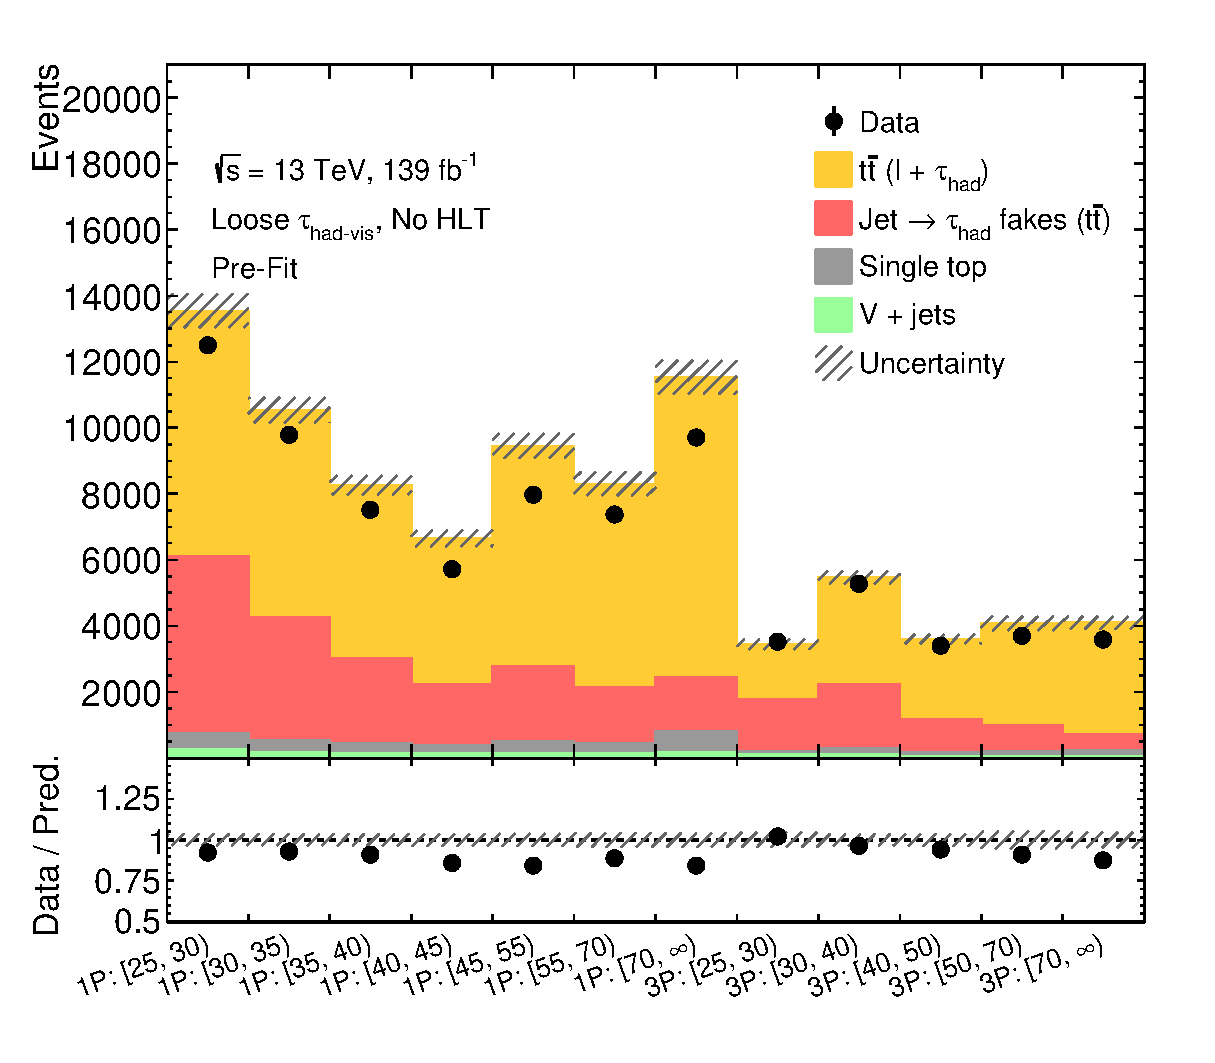
\includegraphics[width=\textwidth]{ttbarSF/Summary_offl}
    \caption{Top control region for events passing the loose
      \tauhadvis identification criteria without trigger-matching.}
  \end{subfigure}\hfill%
  \begin{subfigure}[t]{.485\textwidth}
    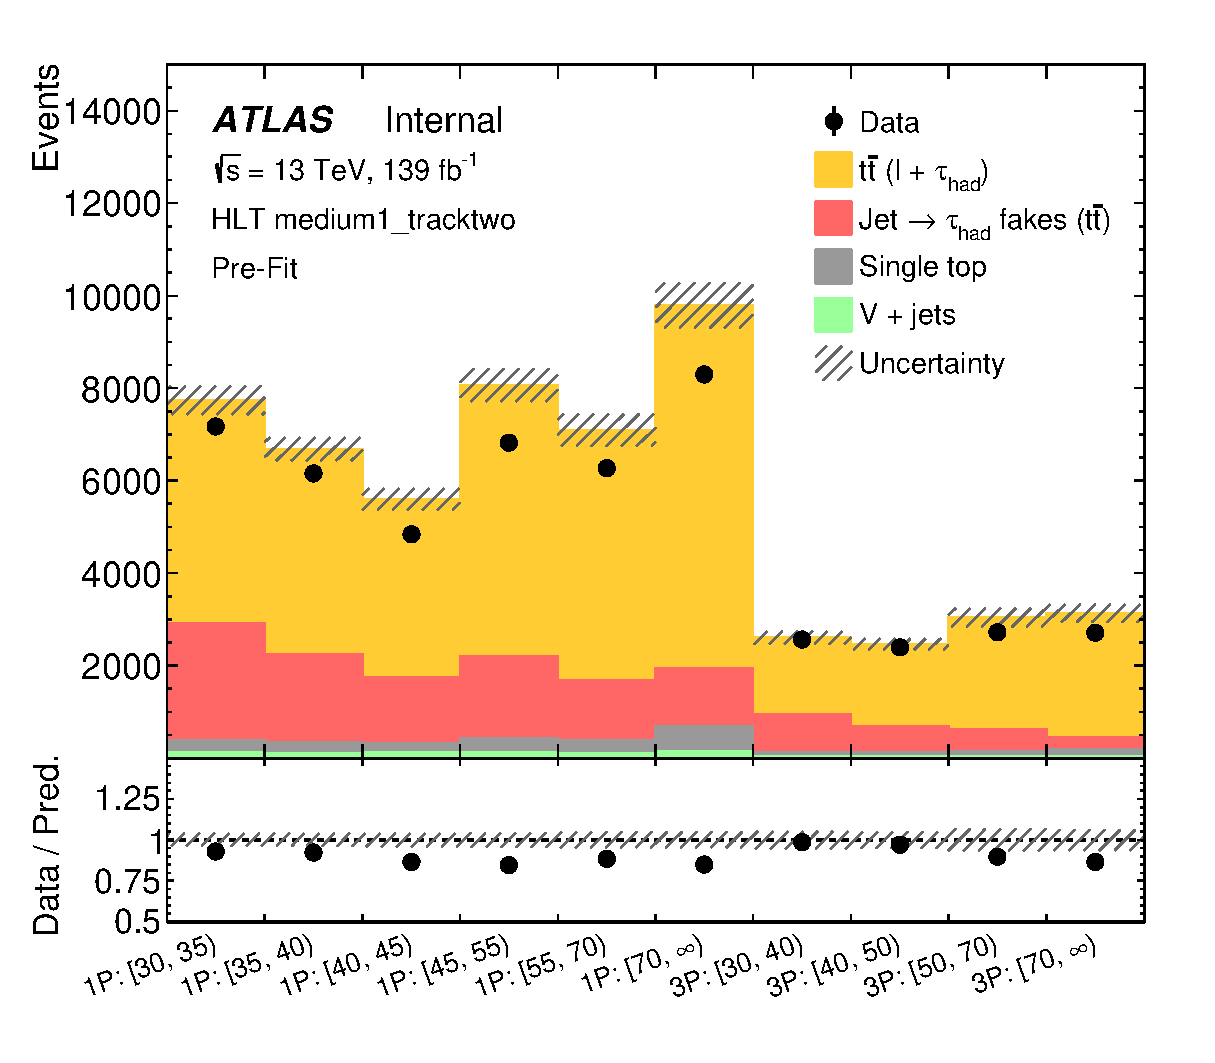
\includegraphics[width=\textwidth]{ttbarSF/Summary_tau25}
    \caption{Top control region for events passing the resurrected
      \texttt{HLT\_tau25\_medium1\_tracktwo} trigger and requiring
      matching between the reconstructed \tauhadvis at HLT and after
      offline \tauhadvis reconstruction.}
  \end{subfigure}

  \caption{Summary of regions used for determination of the \tauhadvis
    misidentification efficiency corrections. The $x$-axis shows the
    regions separated according to the reconstructed decay mode into
    either 1-prong (1P) and 3-prong \tauhadvis as well as the
    \tauhadvis $\pT /\si{\GeV}$ bin interval. The figures are shown
    with the pre-fit background model.}
  \label{fig:ttbarsf_region_summary_prefit}
\end{figure}

The top control region has a large contamination of \ttbar with a
di-lepton final state where the \tauhadvis originates from a \tauhad
decay. This contribution is not sensitive to the jet \ra \tauhadvis
misidentification efficiency but has to be estimated when extracting
correction factors. To distinguish between di-leptonic \ttbar with
true \tauhadvis and (primarily) semi-leptonic \ttbar with
\faketauhadvis, an estimate of the transverse mass between the lepton
$\ell$ and \pTmissAbs (assuming massless daughter particles)
\begin{align*}
  \mTW = \sqrt{2 | \myvec{p}_{\text{T}}^{\ell} | | \pTmiss | \left( 1 - \cos \Delta\phi \right)}
\end{align*}
is used, where $\Delta \phi$ is the angle between the lepton
transverse momentum~$\myvec{p}_{\text{T}}^{\ell}$ and the missing
transverse momentum~\pTmiss.

The distribution of \mTW in the top control region is shown
in~\Cref{fig:ttbarsf_mtw_pdf} inclusive in reconstructed \tauhadvis
decay mode and transverse momentum. The primary source of
\faketauhadvis is \ttbar in a lepton + jets final state which features
a quick reduction in event rate for transverse masses beyond the mass
of the \PW boson. In contrast, \ttbar in the di-lepton final state
shows a comparatively heavy tail towards large values of \mTW due to
the presence of an additional neutrino.

% The main idea is to distinguish between semi-leptonic and di-leptonic
% \ttbar since two true taus would be expected in di-leptonic and jets
% faking taus in semi-leptonic. The all-hadronic mode is negligible due
% to the presence of one electron or muon.

% For semi-leptonic \ttbar the mTW distribution is relatively
% insensitive to the momentum of the tauhadvis candidate. Which is not
% the case for di-leptonic \ttbar.

% For semi-leptonic \ttbar the event rate drops
% significantly beyond \SI{100}{\GeV} while for di-leptonic \ttbar, due
% to the presence of additional neutrinos, the transverse mass extends
% to larger values.


%\Cref{fig:ttbarsf_mtw_examples_prefit}.

\begin{figure}[htbp]
  \centering

  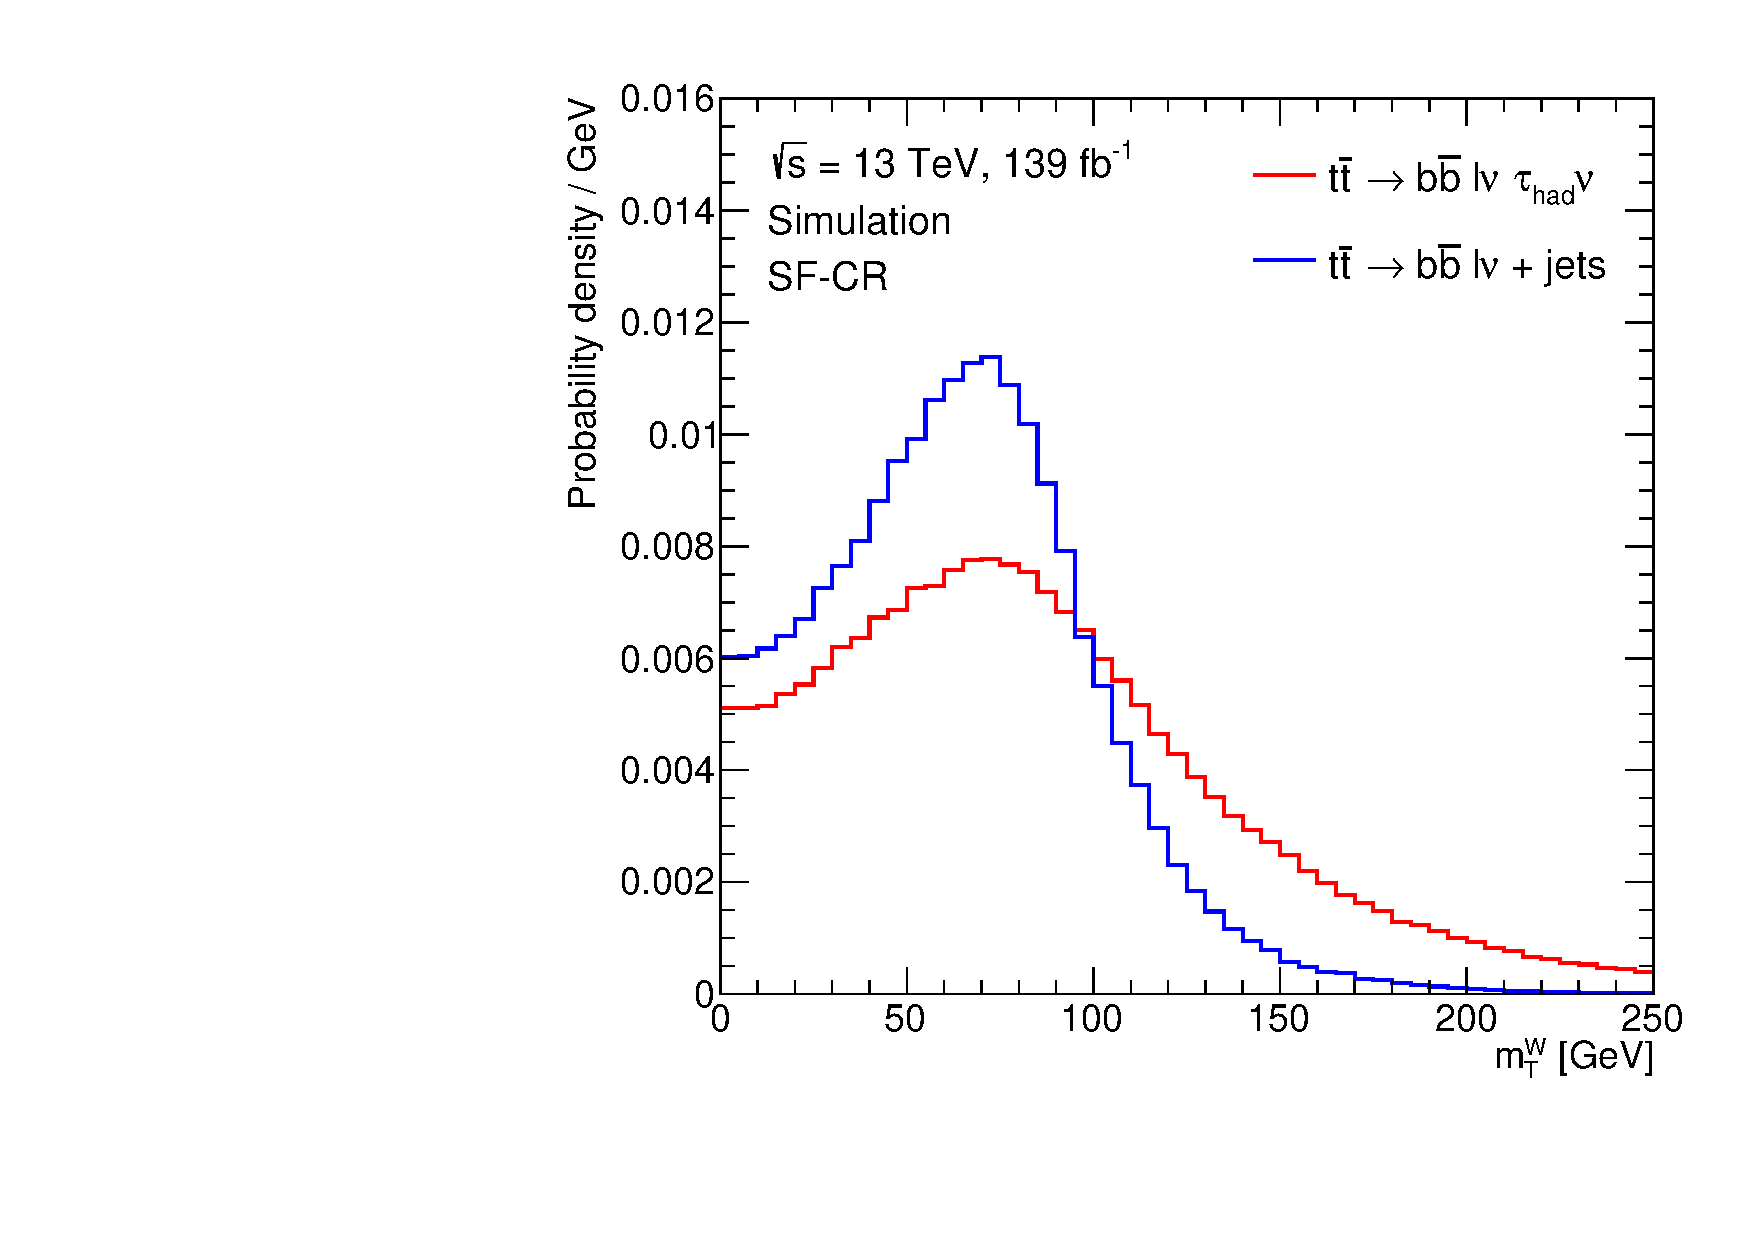
\includegraphics[width=0.45\textwidth]{ttbarSF/mtw_pdf}

  \caption{Transverse mass distribution between lepton and \pTmiss in
    \ttbar simulation. Inclusive in \tauhadvis transverse momentum and
    decay mode. Without applying HLT requirements.}
  \label{fig:ttbarsf_mtw_pdf}
\end{figure}


% To distinguish between semi-leptonic and di-leptonic \ttbar, one can
% try to reconstruct the transverse mass of the \PW boson
% \begin{align*}
%   \mTW = \sqrt{\left( | \myvec{p}_{\text{T}, \ell} | + | \pTmiss | \right)^2
%                - \myvec{p}_{\text{T}, \ell} \cdot \pTmiss}
% \end{align*}
% where $\myvec{p}_{\text{T}, \ell}$ and \pTmiss are the vectors of the
% lepton ($e$ or $\mu$) momentum and missing transverse momentum in the
% transverse plane.









\begin{figure}[htbp]
  \centering

  \begin{subfigure}{.485\textwidth}
    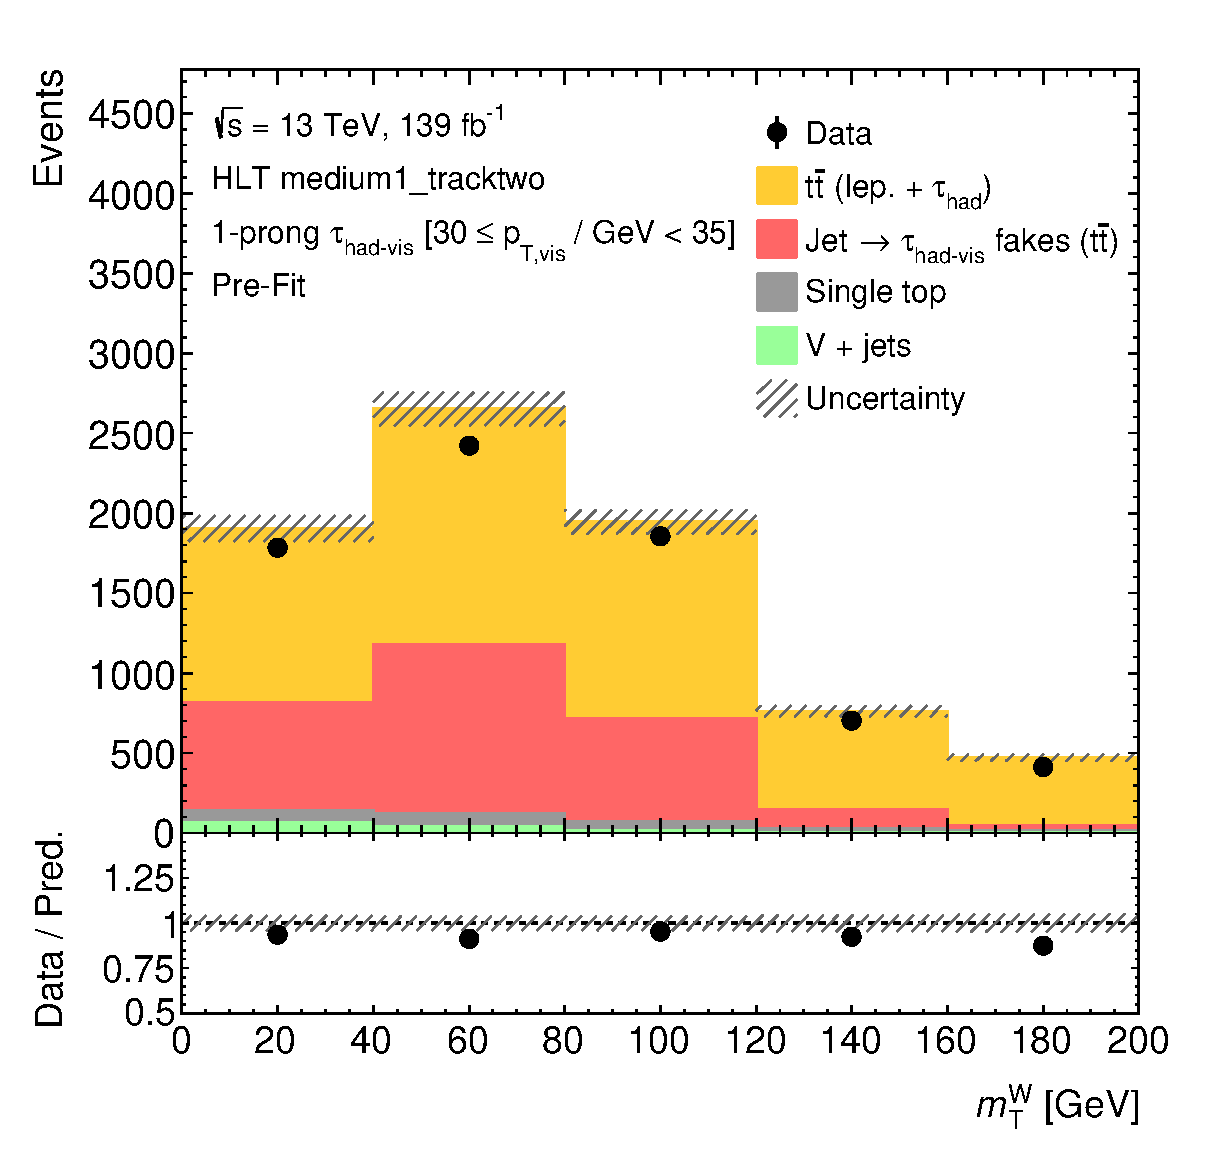
\includegraphics[width=\textwidth]{ttbarSF/tau25/TauPt3035_1P}
    \caption{1-prong \tauhadvis candidates with
      $\SI{30}{\GeV} \leq \pTvis < \SI{35}{\GeV}$.}
  \end{subfigure}\hfill%
  \begin{subfigure}{.485\textwidth}
    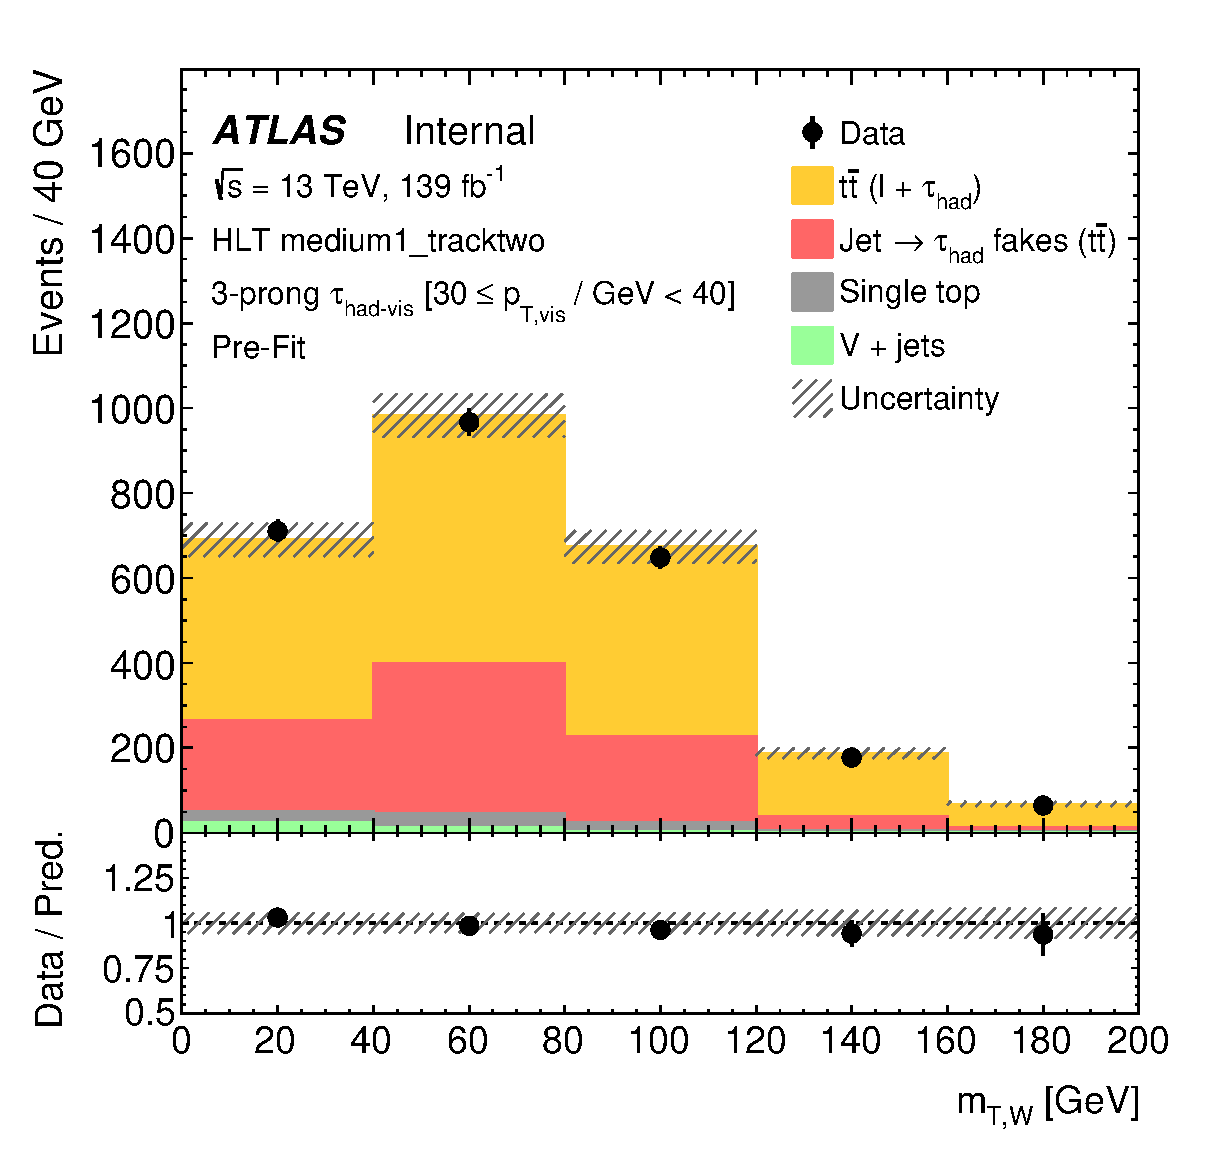
\includegraphics[width=\textwidth]{ttbarSF/tau25/TauPt3040_3P}
    \caption{3-prong \tauhadvis candidates with
      $\SI{30}{\GeV} \leq \pTvis < \SI{40}{\GeV}$.}
  \end{subfigure}

  \caption{Two examples of \mTW distributions. Events with
    $\mTW > \SI{200}{\GeV}$ are merged into the last bin of the
    histogram.}
  \label{fig:ttbarsf_mtw_examples_prefit}
\end{figure}




% Fit model
Fit \mTW

Regions \& normalisation factors






\todo[inline]{Possibly use the SS region to get better constraints on
  ttbar and ttbarFakes.}


\subsubsection{Measurement uncertainties}

To prevent the scale factor measurement from absorbing modelling
issues, systematic uncertainties are applied to the modelling of
\ttbar with true \tauhadvis.


\subsubsection{Application in the analysis}

Propagation of correlations.

How it's applied in \hadhad.

Additional uncertainties.




%%% Local Variables:
%%% mode: latex
%%% TeX-master: "../../phd_thesis"
%%% End:
